\section{Laplace's Equation in Polar Coordinates}

\noindent
In Section~12.3 we solved boundary value
problems for Laplace's equation over a rectangle with sides parallel
to the $x,y$-axes. Now we'll consider boundary value problems for
Laplace's equation over regions with boundaries best described in
terms of polar coordinates. In this case it's appropriate to regard
$u$ as function of $(r,\theta)$ and write Laplace's equation in polar
form as
\begin{equation} \label{eq:12.4.1}
u_{rr}+\frac{1}{r}u_r+\frac{1}{r^2}u_{\theta\theta}=0,
\end{equation}
where
$$
r=\sqrt{x^2+y^2}\mbox{\quad and \quad}
\theta=\cos^{-1}\frac{x}{r}=\sin^{-1}\frac{x}{r}.
$$

We begin with the case where the region
 is a circular disk with radius $\rho$, centered at the origin;   that
is, we want to define a formal solution of the boundary value problem
\begin{equation} \label{eq:12.4.2}
\begin{array}{c}
\dst u_{rr}+\frac{1}{r}u_r+\frac{1}{r^2}u_{\theta\theta}=0,\quad
0<r<\rho,\quad -\pi\le\theta<\pi,\\[2\jot]
u(\rho,\theta)=f(\theta),\quad -\pi\le\theta<\pi
\end{array}
\end{equation}
(Figure~\ref{figure:12.4.1}).
Note that \eqref{eq:12.4.2} imposes no restriction on $u(r,\theta)$
when $r=0$. We'll address this question at
the appropriate time.

\begin{figure}[H]
  \centering\color{blue}
  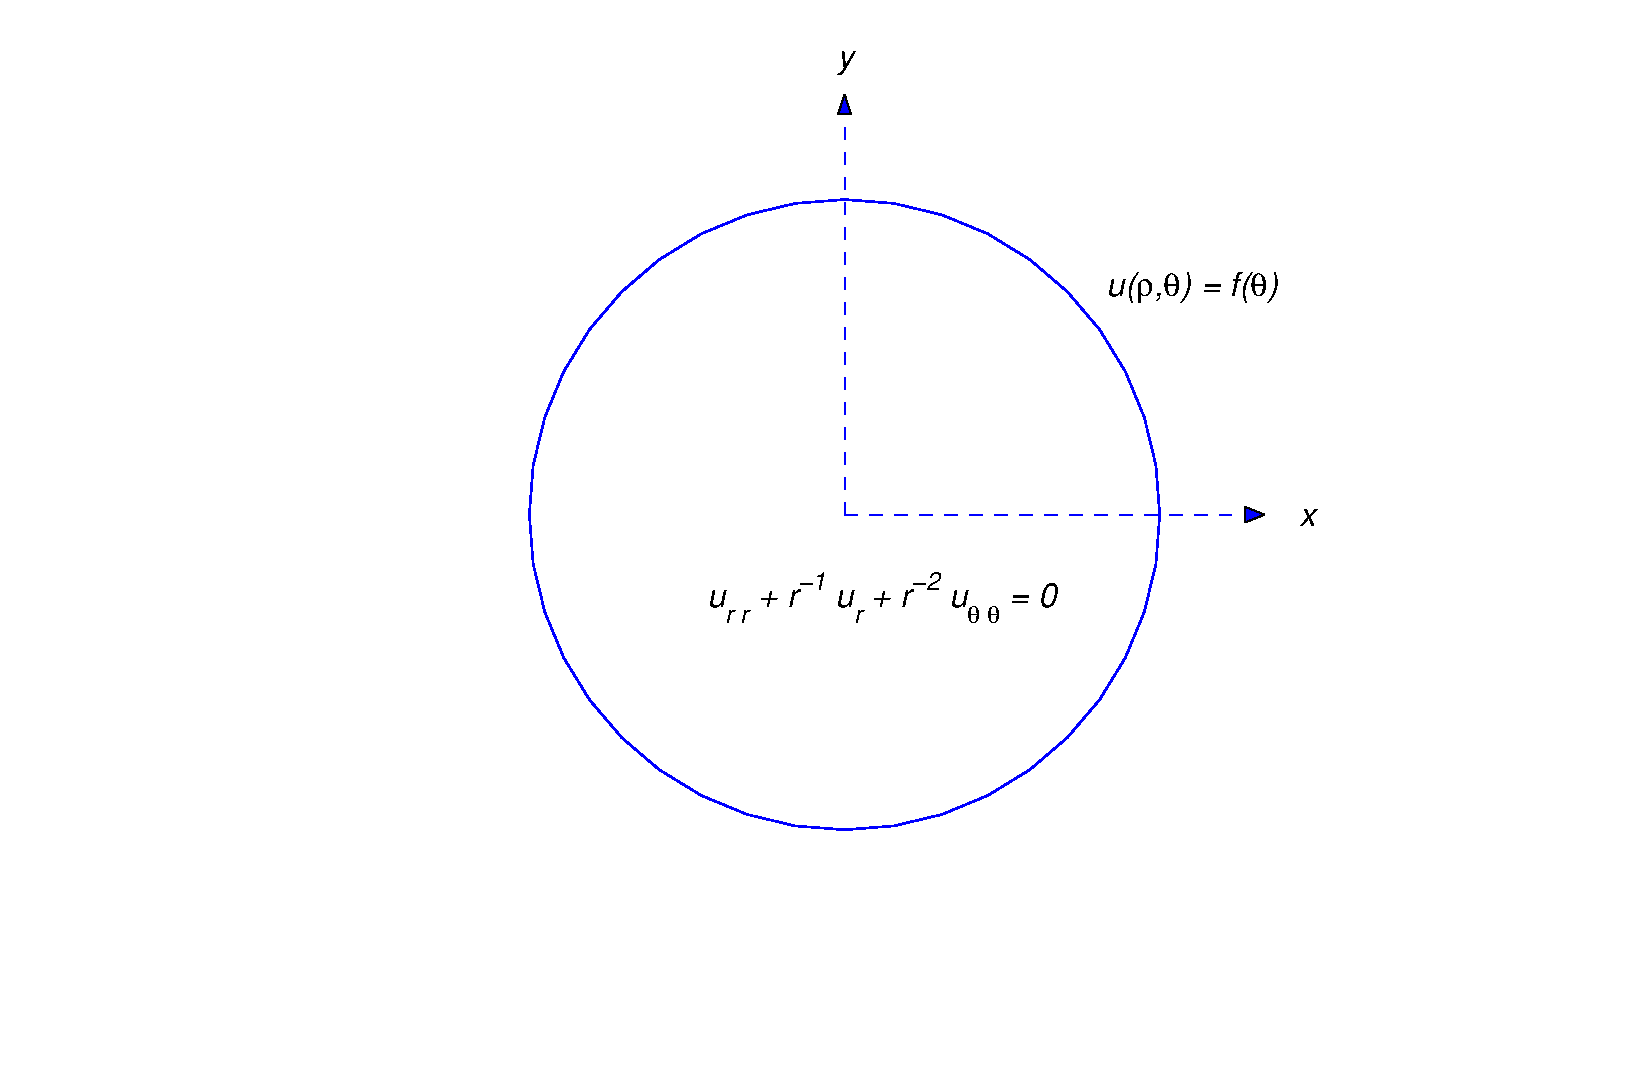
\includegraphics[bb=-78 148 689 643,width=5.67in,height=3.66in,keepaspectratio]{fig120401}
\caption{ The boundary value problem \eqref{eq:12.4.2}}
  \label{figure:12.4.1}
\end{figure}

We first look for products
$v(r,\theta)=R(r)\Theta(\theta)$ that satisfy \eqref{eq:12.4.1}. For
this function,
$$
v_{rr}+\frac{1}{r}v_r+\frac{1}{r^2}v_{\theta\theta}=
R''\Theta+\frac{1}{r}R'\Theta
+\frac{1}{r^2}R\Theta''=0
$$
for all $(r,\theta)$ with $r\ne0$ if
$$
\frac{r^2R''+rR'}{R}=-\frac{\Theta''}{\Theta}=\lambda,
$$
where $\lambda$ is a separation constant. (Verify.)
This equation is equivalent to
$$
\Theta''+\lambda\Theta=0
$$
and
\begin{equation} \label{eq:12.4.3}
r^2R''+rR'-\lambda R=0.
\end{equation}
Since $(r,\pi)$ and $(r,-\pi)$ are the polar coordinates
of the same point, we impose periodic boundary conditions
on $\Theta$; that is,
\begin{equation} \label{eq:12.4.4}
\Theta''+\lambda\Theta=0,\quad \Theta(-\pi)=\Theta(\pi),
\quad \Theta'(-\pi)=\Theta'(\pi).
\end{equation}
Since we don't want  $R\Theta$ to be identically zero,
$\lambda$ must be an eigenvalue of \eqref{eq:12.4.4} and $\Theta$
must be an associated eigenfunction. From Theorem~\ref{thmtype:11.1.6},
the eigenvalues of \eqref{eq:12.4.4} are $\lambda_0=0$ with
associated eigenfunctions $\Theta_0=1$ and, for $n=1,2,3,\dots,$
$\lambda_n=n^2$,
with associated eigenfunction $\cos n\theta$ and $\sin n\theta$
therefore,
$$
 \Theta_n=\alpha_n\cos n\theta+\beta_n\sin n\theta
$$
where $\alpha_n$ and $\beta_n$ are constants.

Substituting $\lambda=0$ into \eqref{eq:12.4.3} yields the
$$
r^2R''+rR'=0,
$$
so
$$
\frac{R_0''}{R_0'}=-\frac{1}{r},
$$
$$
R_0'=\frac{c_1}{r},
$$
and
\begin{equation} \label{eq:12.4.5}
R_0=c_2+c_1\ln r.
\end{equation}
If $c_1\ne0$ then
$$
\lim_{r\to0+}|R_0(r)|=\infty,
$$
which doesn't make sense if we interpret
$u_0(r,\theta)=R_0(r)\Theta_0(\theta)=R_0(r)$ as the steady state
temperature distribution in a disk whose boundary is maintained
at the constant temperature $R_0(\rho)$.
Therefore we now require
$R_0$ to be bounded as $r\to0+$.  This implies that $c_1=0$, and
we  take $c_2=1$.
Thus, $R_0=1$ and $v_0(r,\theta)=R_0(r)\Theta_0(\theta)=1$.
Note that $v_0$ satisfies \eqref{eq:12.4.2} with
$f(\theta)=1$.

Substituting $\lambda=n^2$ into \eqref{eq:12.4.3} yields
the Euler equation
\begin{equation} \label{eq:12.4.6}
r^2R_n''+rR_n'-n^2 R_n=0
\end{equation}
for $R_n$.
The indicial polynomial of this equation is
$$
s(s-1)+s-n^2=(s-n)(s+n),
$$
so the general solution of \eqref{eq:12.4.6} is
\begin{equation} \label{eq:12.4.7}
R_n=c_1r^n+c_2r^{-n},
\end{equation}
by Theorem~\ref{thmtype:7.4.3}. Consistent with our previous assumption on
$R_0$, we now require  $R_n$  to be bounded as $r\to0+$.
This implies that  $c_2=0$, and we   choose
$c_1=\rho^{-n}$.
Then
$R_n(r)=r^n/\rho^n$, so
$$
v_n(r,\theta)=R_n(r)\Theta_n(\theta)=\frac{r^n}{\rho^n}(\alpha_n\cos
n\theta+\sin n\theta).
$$
Now  $v_n$ satisfies \eqref{eq:12.4.2} with
$$
f(\theta)=\alpha_n\cos n\theta+\beta_n\sin n\theta.
$$
More generally, if $\alpha_0$, $\alpha_1$,\dots, $\alpha_m$ and
$\beta_1$,
$\beta_2$,
\dots, $\beta_m$ are arbitrary constants then
$$
u_m(r,\theta)=\alpha_0+\sum_{n=1}^m\frac{r^n}{\rho^n}(\alpha_n\cos
n\theta+\beta_n\sin n\theta)
$$
satisfies \eqref{eq:12.4.2} with
$$
f(\theta)
=\alpha_0+\sum_{n=1}^m(\alpha_n\cos
n\theta+\beta_n\sin n\theta).
$$
This motivates the next definition.

\begin{definition}\color{blue} \label{thmtype:12.4.1} \rm
The bounded formal solution of the boundary value problem
\eqref{eq:12.4.2} is
\begin{equation} \label{eq:12.4.8}
u(r,\theta)=\alpha_0+\sum_{n=1}^\infty\frac{r^n}{\rho^n}(\alpha_n\cos
n\theta+\beta_n\sin n\theta),
\end{equation}
where
$$
F(\theta)
=\alpha_0+\sum_{n=1}^\infty(\alpha_n\cos
n\theta+\beta_n\sin n\theta)
$$
is the Fourier series of  $f$ on $[-\pi,\pi]$; that is,
$$
\alpha_0=\frac{1}{2\pi}\int_{-\pi}^\pi f(\theta)\,d\theta,
$$
and
$$
\alpha_n=\frac{1}{\pi}\int_{-\pi}^\pi f(\theta)\cos n\theta\,d\theta
\text{\quad and \quad}
\beta_n=\frac{1}{\pi}\int_{-\pi}^\pi f(\theta)\sin
n\theta\,d\theta,
\quad n=1,2,3,\dots.
$$
\end{definition}

Since $\sum_{n=0}^\infty n^k(r/\rho)^n$  converges for every
$k$ if $0< r<\rho$, Theorem~\ref{thmtype:12.1.2} can be used to show that if
$0< r<\rho$ then
 \eqref{eq:12.4.8} can be differentiated term by term
any number of times with respect to both $r$ and $\theta$.
Since the  terms in \eqref{eq:12.4.8} satisfy Laplace's
equation if $r>0$,  \eqref{eq:12.4.8} satisfies
Laplace's equation if $0<r<\rho$. Therefore, since
$u(\rho,\theta)=F(\theta)$,
$u$ is an actual solution of \eqref{eq:12.4.2} if and only if
$$
F(\theta)=f(\theta),\quad -\pi\le\theta<\pi.
$$
From Theorem~\ref{thmtype:11.2.4}, this is true if $f$ is continuous and piecewise
smooth on $[-\pi,\pi]$ and $f(-\pi)=f(\pi)$.

\begin{example}\label{example:12.4.1} \rm
Find the bounded formal solution of \eqref{eq:12.4.2} with
$f(\theta)=\theta(\pi^2-\theta^2)$.
\end{example}

\solution From  Example~\ref{example:11.2.6},
$$
\theta(\pi^2-\theta^2)=12\sum_{n=1}^\infty\frac{(-1)^n}{n^3}\sin
n\theta,\quad -\pi\le\theta\le\pi,
$$
so
$$
u(r,\theta)=12\sum_{n=1}^\infty\frac{r^n}{\rho^n}\frac{(-1)^n}{n^3}\sin
n\theta,\quad
0\le r\le \rho,\quad -\pi\le\theta\le\pi.
$$

\begin{example}\label{example:12.4.2} \rm
Define the formal solution of
\begin{equation} \label{eq:12.4.9}
\begin{array}{c}
\dst u_{rr}+\frac{1}{r}u_r+\frac{1}{r^2}u_{\theta\theta}=0,\quad
\rho_0<r<\rho,\quad -\pi\le\theta<\pi,\\[2\jot]
u(\rho_0,\theta)=0,\quad  u(\rho,\theta)=f(\theta),\quad
-\pi\le\theta<\pi,
\end{array}
\end{equation}
where $0<\rho_0<\rho$ (Figure~\ref{figure:12.4.2}).
\end{example}

 \begin{figure}[H]
  \centering\color{blue}
  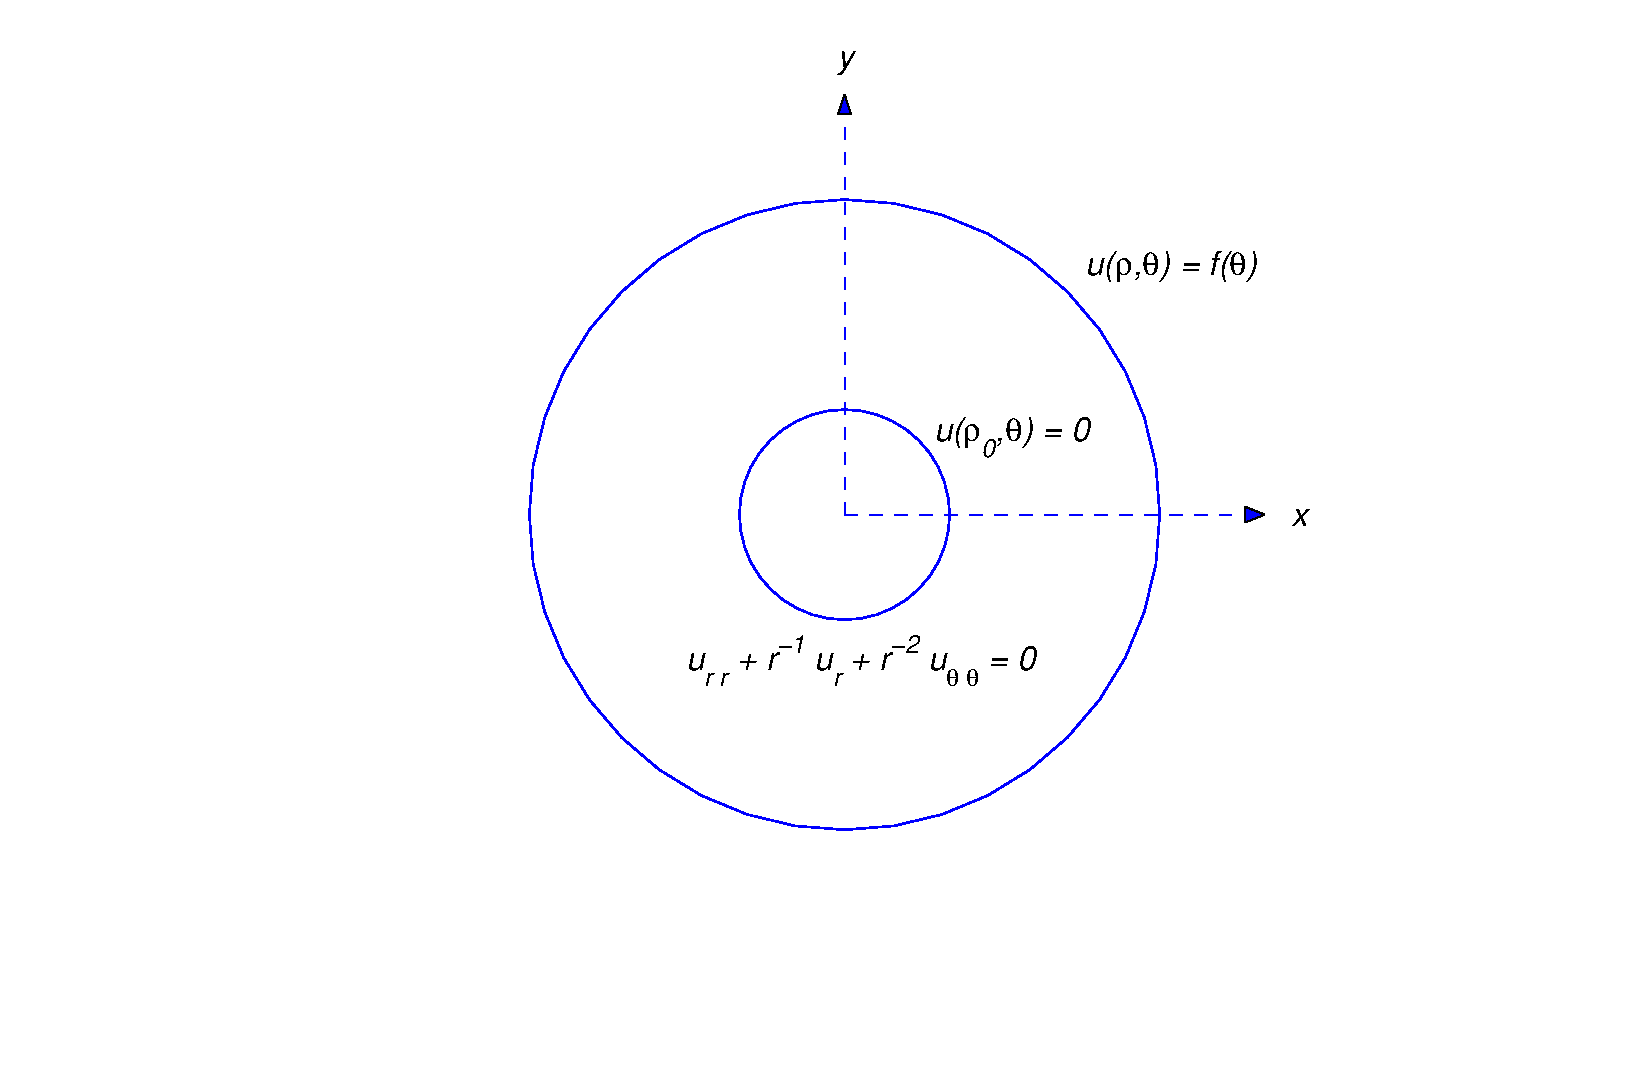
\includegraphics[bb=-78 148 689 643,width=5.67in,height=3.66in,keepaspectratio]{fig120402}
\caption{ The boundary value problem \eqref{eq:12.4.9}}
  \label{figure:12.4.2}
\end{figure}

\solution
We use separation of variables exactly as before, except that
now we choose the constants in \eqref{eq:12.4.5} and \eqref{eq:12.4.7}
so that $R_n(\rho_0)=0$ for $n=0$, $1$, $2$,\dots. In view of the
nonhomogeneous Dirichlet
condition on the boundary $r=\rho$, it's also convenient to require
that
$R_n(\rho)=1$ for $n=0$, $1$, $2$,\dots. We leave it to you to verify
that
$$
R_0(r)=\frac{\ln r/\rho_0}{\ln\rho/\rho_0}
\mbox{\quad and \quad}
R_n=\frac{\rho_0^{-n}r^n-\rho_0^nr^{-n}}
{\rho_0^{-n}\rho^n-\rho_0^n\rho^{-n}},\quad n=1,2,3,\dots
$$
satisfy these requirements. Therefore
$$
v_0(\rho,\theta)=\frac{\ln r/\rho_0}{\ln\rho/\rho_0}
$$
and
$$
v_n(r,\theta)=\frac{\rho_0^{-n}r^n-\rho_0^nr^{-n}}
{\rho_0^{-n}\rho^n-\rho_0^n\rho^{-n}}(\alpha_n\cos n\theta+\beta_n\sin
n\theta),
\quad n=1,2,3,\dots,
$$
where $\alpha_n$ and $\beta_n$ are arbitrary constants.

If $\alpha_0$, $\alpha_1$,\dots, $\alpha_m$ and
$\beta_1$,
$\beta_2$,
\dots, $\beta_m$ are arbitrary constants then
$$
u_m(r,\theta)=\alpha_0\frac{\ln r/\rho_0}{\ln\rho/\rho_0}+
\sum_{n=1}^m
\frac{\rho_0^{-n}r^n-\rho_0^nr^{-n}}
{\rho_0^{-n}\rho^n-\rho_0^n\rho^{-n}}
(\alpha_n\cos
n\theta+\beta_n\sin n\theta)
$$
satisfies \eqref{eq:12.4.9}, with
$$
f(\theta)
=\alpha_0+\sum_{n=1}^m(\alpha_n\cos
n\theta+\beta_n\sin n\theta).
$$
This motivates us to define the formal solution of \eqref{eq:12.4.9}
for general $f$ to be
$$
u(r,\theta)=\alpha_0\frac{\ln r/\rho_0}{\ln\rho/\rho_0}+
\sum_{n=1}^\infty
\frac{\rho_0^{-n}r^n-\rho_0^nr^{-n}}
{\rho_0^{-n}\rho^n-\rho_0^n\rho^{-n}}
(\alpha_n\cos
n\theta+\beta_n\sin n\theta),
$$
where
$$
F(\theta)
=\alpha_0+\sum_{n=1}^\infty(\alpha_n\cos
n\theta+\beta_n\sin n\theta)
$$
is the Fourier series of  $f$ on $[-\pi,\pi]$.

\begin{example}\label{example:12.4.3} \rm
Define the bounded formal solution of
\begin{equation} \label{eq:12.4.10}
\begin{array}{c}
\dst u_{rr}+\frac{1}{r}u_r+\frac{1}{r^2}u_{\theta\theta}=0,\quad
0<r<\rho,\quad 0<\theta<\gamma,\\[2\jot]
 u(\rho,\theta)=f(\theta),\quad 0\le\theta\le\gamma,\\[2\jot]
u(r,0)=0,\quad u(r,\gamma)=0,\quad 0<r<\rho,
\end{array}
\end{equation}
where $0<\gamma<2\pi$ (Figure~\ref{figure:12.4.3}).
\end{example}

\begin{figure}[tbp]
  \centering\color{blue}
  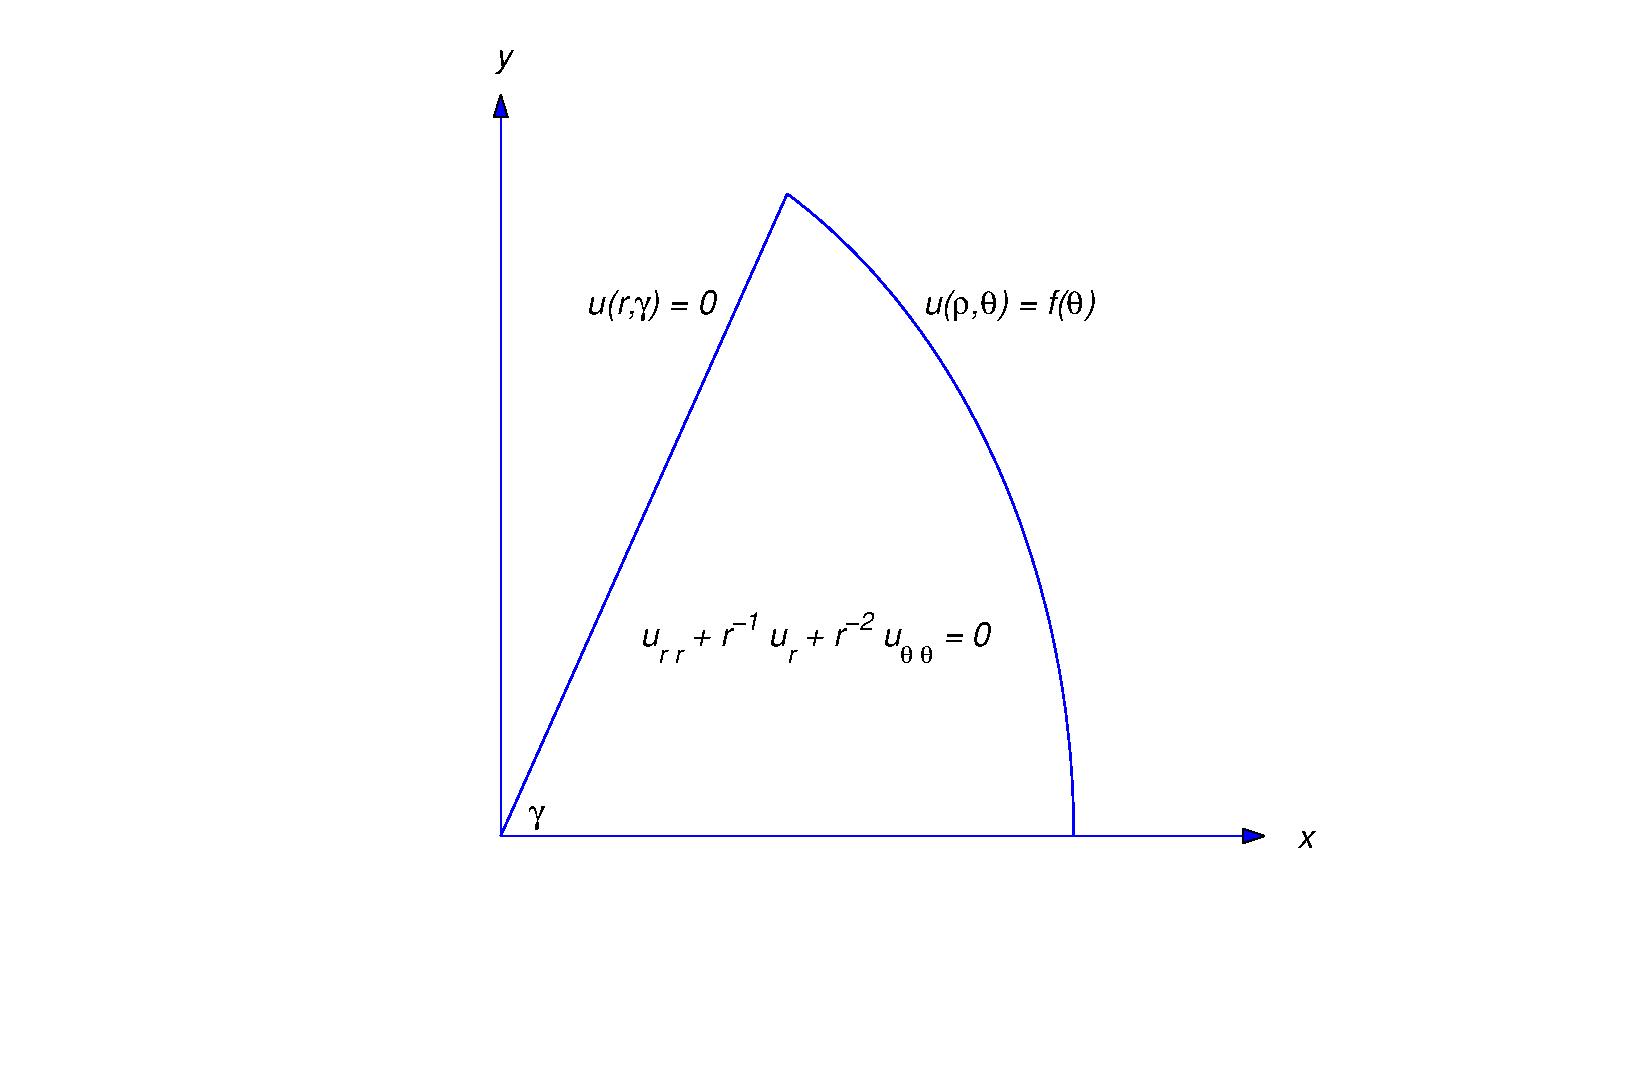
\includegraphics[bb=-78 148 689 643,width=5.67in,height=3.66in,keepaspectratio]{fig120403}
\caption{ The boundary value problem \eqref{eq:12.4.10}}
  \label{figure:12.4.3}
\end{figure}

\solution
Now $v(r,\theta)=R(r)\Theta(\theta)$, where
\begin{equation} \label{eq:12.4.11}
r^2R''+rR'-\lambda R=0
\end{equation}
and
\begin{equation} \label{eq:12.4.12}
\Theta''+\lambda\Theta=0,\quad \Theta(0)=0,\quad \Theta(\gamma)=0.
\end{equation}
From Theorem~\ref{thmtype:11.1.2},
the eigenvalues of \eqref{eq:12.4.12}  are
$\lambda_n=n^2\pi^2/\gamma^2$,
with associated eigenfunction $\Theta_n=\sin n\pi\theta/\gamma$,
$n=1$,  $2$, $3$,\dots.
Substituting $\lambda=n^2\pi^2/\gamma^2$ into \eqref{eq:12.4.11} yields
the Euler equation
$$
r^2R''+rR_n'-\frac{n^2\pi^2}{\gamma^2} R=0.
$$
The indicial polynomial of this equation is
$$
s(s-1)+s-\frac{n^2\pi^2}{\gamma^2}=\left(s-\frac{n\pi}{\gamma}\right)
\left(s+\frac{n\pi}{\gamma}\right),
$$
so
$$
R_n=c_1r^{n\pi/\gamma}+c_2r^{-n\pi/\gamma},
$$
by Theorem~\ref{thmtype:7.4.3}.
To obtain a solution that remains bounded as
$r\to0+$ we let $c_2=0$. Because of the Dirichlet condition at
$r=\rho$, it's convenient to have $r(\rho)=1$;   therefore we take
$c_1=\rho^{-n\pi/\gamma}$, so
$$
R_n(r)=\frac{r^{n\pi/\gamma}}{\rho^{n\pi/\gamma}}.
$$
Now
$$
v_n(r,\theta)=R_n(r)\Theta_n(\theta)=\frac{r^{n\pi/\gamma}}
{\rho^{n\pi/\gamma}}\sin\frac{n\pi\theta}{\gamma}
$$
 satisfies \eqref{eq:12.4.10} with
$$
f(\theta)=\sin\frac{n\pi\theta}{\gamma}.
$$
More generally, if  $\alpha_1$, $\alpha_2$, \dots, $\alpha_m$ and
 are arbitrary constants then
$$
u_m(r,\theta)=\sum_{n=1}^m\alpha_n\frac{r^{n\pi/\gamma}}{\rho^{n\pi/\gamma}}
\sin\frac{n\pi\theta}{\gamma}
$$
satisfies \eqref{eq:12.4.10} with
$$
f(\theta)
=\sum_{n=1}^m\alpha_n\sin\frac{n\pi\theta}{\gamma}.
$$
This motivates us to define the bounded formal solution of
\eqref{eq:12.4.10} to be
$$
u_m(r,\theta)=\sum_{n=1}^\infty\alpha_n\frac{r^{n\pi/\gamma}}{\rho^{n\pi/\gamma}}
\sin\frac{n\pi\theta}{\gamma},
$$
where
$$
S(\theta)=\sum_{n=1}^\infty\alpha_n
\sin\frac{n\pi\theta}{\gamma}
$$
is the Fourier sine expansion of $f$ on $[0,\gamma]$; that is,
$$
\alpha_n=\frac{2}{\gamma}\int_0^\gamma
f(\theta)\sin\frac{n\pi\theta}{\gamma}\,d\theta.
$$

\exercises
\begin{exerciselist}

\item\label{exer:12.4.1}
Define the formal solution of
$$
\begin{array}{c}
\dst u_{rr}+\frac{1}{r}u_r+\frac{1}{r^2}u_{\theta\theta}=0,\quad
\rho_0<r<\rho,\quad -\pi\le\theta<\pi,\\[2\jot]
u(\rho_0,\theta)=f(\theta),\quad  u(\rho,\theta)=0,\quad
-\pi\le\theta<\pi,
\end{array}
$$
where $0<\rho_0<\rho$.

\item\label{exer:12.4.2}
Define the  formal solution of
$$
\begin{array}{c}
\dst u_{rr}+\frac{1}{r}u_r+\frac{1}{r^2}u_{\theta\theta}=0,\quad
\rho_0<r<\rho,\quad 0<\theta<\gamma,\\[2\jot]
u(\rho_0,\theta)=0,\quad  u(\rho,\theta)=f(\theta),\quad
0\le\theta\le\gamma,\\[2\jot]
u(r,0)=0,\quad u(r,\gamma)=0,\quad \rho_0<r<\rho,
\end{array}
$$
where $0<\gamma<2\pi$ and $0<\rho_0<\rho$.

\item\label{exer:12.4.3}
Define the  formal solution of
$$
\begin{array}{c}
\dst u_{rr}+\frac{1}{r}u_r+\frac{1}{r^2}u_{\theta\theta}=0,\quad
\rho_0<r<\rho,\quad 0<\theta<\gamma,\\[2\jot]
u(\rho_0,\theta)=0,\quad  u_r(\rho,\theta)=g(\theta),\quad
0\le\theta\le\gamma,\\[2\jot]
u_\theta(r,0)=0,\quad u_\theta(r,\gamma)=0,\quad \rho_0<r<\rho,
\end{array}
$$
where $0<\gamma<2\pi$ and $0<\rho_0<\rho$.

\item\label{exer:12.4.4}
Define the bounded formal solution of
$$
\begin{array}{c}
\dst u_{rr}+\frac{1}{r}u_r+\frac{1}{r^2}u_{\theta\theta}=0,\quad
0<r<\rho,\quad 0<\theta<\gamma,\\[2\jot]
  u(\rho,\theta)=f(\theta),\quad
0\le\theta\le\gamma,\\[2\jot]
u_\theta(r,0)=0,\quad u(r,\gamma)=0,\quad 0<r<\rho,
\end{array}
$$
where $0<\gamma<2\pi$.

\item\label{exer:12.4.5}
Define the  formal solution of
$$
\begin{array}{c}
\dst u_{rr}+\frac{1}{r}u_r+\frac{1}{r^2}u_{\theta\theta}=0,\quad
\rho_0<r<\rho,\quad 0<\theta<\gamma,\\[2\jot]
u_r(\rho_0,\theta)=g(\theta),\quad
u_r(\rho,\theta)=0,\quad
0\le\theta\le\gamma,\\[2\jot]
u(r,0)=0,\quad u_\theta(r,\gamma)=0,\quad \rho_0<r<\rho,
\end{array}
$$
where $0<\gamma<2\pi$ and $0<\rho_0<\rho$.

\item\label{exer:12.4.6}
Define the bounded formal solution of
$$
\begin{array}{c}
\dst u_{rr}+\frac{1}{r}u_r+\frac{1}{r^2}u_{\theta\theta}=0,\quad
0<r<\rho,\quad 0<\theta<\gamma,\\[2\jot]
  u(\rho,\theta)=f(\theta),\quad
0\le\theta\le\gamma,\\[2\jot]
u_\theta(r,0)=0,\quad u_\theta(r,\gamma)=0,\quad 0<r<\rho,
\end{array}
$$
where $0<\gamma<2\pi$.

\item\label{exer:12.4.7}
Show that the Neumann problem
$$
\begin{array}{c}
\dst u_{rr}+\frac{1}{r}u_r+\frac{1}{r^2}u_{\theta\theta}=0,\quad
0<r<\rho,\quad -\pi\le\theta<\pi,\\[2\jot]
u_r(\rho,\theta)=f(\theta),\quad -\pi\le\theta<\pi
\end{array}
$$
has no bounded formal solution unless $\int_{-\pi}^\pi
f(\theta)\,d\theta=0$.   In this case it has infinitely many
solutions. Find those solutions.

\end{exerciselist}

